\documentclass[9pt]{beamer}


\usepackage[font=footnotesize,labelfont=bf]{caption}
\usepackage[RPvoltages]{circuitikz}
\usepackage[T1]{fontenc}
\usepackage[short]{optidef}
\usepackage[short]{optidef}
\usepackage{adjustbox}
\usepackage{algorithm}
\usepackage{algpseudocode}
\usepackage{amsfonts}
\usepackage{amsmath}
\usepackage{amssymb}
\usepackage{amsthm}
\usepackage{array}
\usepackage{cite}
\usepackage{cuted}
\usepackage{environ}
\usepackage{grffile}
\usepackage{hyperref}
\usepackage{import}
\usepackage{lmodern}
\usepackage{mathtools}
\usepackage{microtype}
\usepackage{multirow}
\usepackage{pgfgantt}
\usepackage{pgfplots}
\usepackage{physics}
\usepackage{siunitx}
\usepackage{stfloats}
\usepackage{subcaption}
\usepackage{url}
\usepackage{xcolor}


\interdisplaylinepenalty=2500
\pgfplotsset{compat=newest}
\usetikzlibrary{plotmarks}
\usetikzlibrary{arrows.meta}
\usepgfplotslibrary{patchplots}
\newtheorem{proposition}{Proposition}
\DeclareSIUnit{\belm}{Bm}
\DeclareSIUnit{\dBm}{\deci\belm}
\DeclareSIUnit{\beli}{Bi}
\DeclareSIUnit{\dBi}{\deci\beli}

\makeatletter
\newcommand{\forcealgorithm}{\let\@latex@error\@gobble}
\makeatother

\usepackage{siunitx}
\DeclareSIUnit{\belmilliwatt}{Bm}
\DeclareSIUnit{\dBm}{\deci\belmilliwatt}

\usepackage{blindtext}
\newcommand\blfootnote[1]{%
\begingroup
\renewcommand\thefootnote{}\footnote{#1}%
\addtocounter{footnote}{-1}%
\endgroup
}

\usetheme{Warsaw}
\setbeamerfont{subsection in toc}{size=\footnotesize}

\AtBeginSection
{
    \begin{frame}
        \frametitle{Table of Contents}
        \tableofcontents[currentsection]
    \end{frame}
}

\title{Symbiotic Radio: \\Towards Spectrum and Energy Efficient Transmission}
\author{Yang Zhao}
\institute{Department of Electrical and Electronic Engineering\\ Imperial College London}
\date{Tech rewiew, \today}

\begin{document}

	% \begin{abstract}
	% 	Symbiotic Radio (SR) enables a secondary transmission over the primary link in a fully passive manner. In today's tech review, we will briefly introduce backscatter basics and see how SR uses the spectrum and energy efficiently.
	% \end{abstract}

	\frame{\titlepage}

	\begin{section}{Introduction to Backscatter Communication}
		\begin{subsection}{Antennas: Transmitter vs Scatterer}
			\begin{frame}{Antennas: Transmitter vs Scatterer}
				\textbf{Green's decomposition:} the (back)scattered signal of an antenna can be decomposed into \textit{structural mode} component and \textit{antenna mode} component.
				\begin{figure}[!t]
					\centering
					\subfloat[Transmit antenna\label{ci:transmit_antenna}]{
						\resizebox{0.2\columnwidth}{!}{
							\begin{circuitikz}[transform shape]
								\draw (0,0) node[ground](GND){} to [R=$Z_{\text{L}}$,-*] (0,2);
								\draw (0,2) to [R=$Z_{\text{ant}}$] (0,4) node[bareantenna](bareantenna){};
								\draw (bareantenna.west) +(-1,0) node[waves,opacity=0]{};
								\draw (bareantenna.east) +(0.7,0) node[waves]{$E_{\text{tx}}$};
							\end{circuitikz}
						}
					}
					\subfloat[Backscatter antenna\label{ci:backscatter_antenna}]{
						\resizebox{0.2\columnwidth}{!}{
							\begin{circuitikz}[transform shape]
								\draw (0,0) node[ground](GND){};
								\draw (0,2) node[spdt,rotate=270](SW){};
								\draw (GND -| SW.out 1) to (GND -| SW.out 2);
								\draw (GND -| SW.out 2) to [R=$Z_{\text{L,}1}$] (SW.out 2);
								\draw (GND -| SW.out 1) to [R,l_=$Z_{\text{L,}2}$] (SW.out 1);
								\draw (SW.in) to [R=$Z_{\text{ant}}$] (0,4) node[bareantenna](bareantenna){};
								\draw (bareantenna.west) +(-1,0) node[waves]{$E_{\text{inc}}$};
								\draw (bareantenna.east) +(0.7,0) node[waves]{$E_{\text{scat}}$};
							\end{circuitikz}
						}
					}
				\end{figure}
				\begin{equation}
					E_{\text{scat}}(Z_{\text{L}})=\underbrace{E_{\text{scat}}(Z_{\text{ant}}^*)}_{\text{structural mode, fixed}}+\underbrace{\alert{\Gamma^*}E_{\text{ant}}\frac{I_{\text{m}}^*}{I_{\text{ant}}}}_{\text{antenna mode, adjustable}}
				\end{equation}
			\end{frame}
		\end{subsection}

		\begin{subsection}{Backscatter Modulation}
			\begin{frame}{Non-Frequency Shifting Modulation}
				\textbf{Non-Frequency Shifting (FS) modulation} only changes the amplitude and phase of the incident signal. The backscattered signal can be controlled by varying the load at the reflector.
				\begin{equation}
					\Gamma^*(Z_{\text{L}})=\frac{Z_{\text{ant}}^*-Z_{\text{L}}}{Z_{\text{ant}}+Z_{\text{L}}}
				\end{equation}

				\vspace{1em}

				Key issue: design a reflection coefficient set corresponding to the signal constellation set $\mathcal{C}$. For each constellation point $c_i \in \mathcal{C}$,
				\begin{equation}
					\Gamma_i=\alpha \frac{c_i}{\max_{c \in \mathcal{C}}\lvert{c}\rvert}
				\end{equation}
				where the constant $\alpha<1$ determines the tradeoff between \textit{backscatter strength} and \textit{harvestable power} at the reflector.
			\end{frame}

			\begin{frame}{Frequency Shifting Modulation}
				\textbf{Frequency shifting modulation} changes $\Gamma$ over time to approximate a sine wave $ce^{j2 \pi \Delta ft}=c\left(\cos(j2 \pi \Delta ft)+j\sin(j2 \pi \Delta ft)\right)$\footnote{In practice, the sin/cos terms can be approximated by a convenient square wave (large amplitude at $\Delta f$, small interference at harmonics)}.

				\vspace{1em}

				For a incoming signal $\cos(2 \pi ft)$, the backscattered signal is
				\begin{equation}
					ce^{j2 \pi \Delta ft} \cos(2 \pi ft) = \frac{c}{2}(\underbrace{e^{j2 \pi (f + \Delta f)t}}_{\text{desired}}+\underbrace{e^{j2 \pi (-f + \Delta f)t}}_{\text{mirror}})
				\end{equation}

				Some modulation techniques (e.g. inter-technology backscatter \cite{Iyer2016}, HitchHike \cite{Zhang2016a}) can be used to suppress the mirror copy.

				\begin{figure}
					\centering
					\includegraphics[width=\textwidth]{assets/fs_backscatter.png}
					\caption{Incident and backscattered waveform \cite{Iyer2016,Kellogg2016}}
					\label{fi:fs_backscatter}
				\end{figure}
			\end{frame}
		\end{subsection}

		\begin{subsection}{Backscatter Techniques}
			\begin{frame}{Ambient Backscatter Communication}
				\textbf{Ambient Backscatter Communication (AmBC)} utilizes the surrounding RF signals (e.g. TV, Wi-Fi) to enable communications between batteryless devices.

				\begin{figure}
					\centering
					\includegraphics[width=0.6\textwidth]{assets/ambient_backscatter_system.png}
					\caption{An ambient backscatter communication system \cite{Zhao2017}}
					\label{fi:ambient_backscatter}
				\end{figure}

				The passive tag harvests energy from and modulate over the ambient RF signal.
			\end{frame}

			\begin{frame}{Intelligent Reflecting Surface}
				\textbf{Intelligent Reflecting Surface (IRS)} consists of multiple individual passive reflecting elements that adjust the amplitude and phase of the incident signal.
				\begin{figure}
					\centering
					\begin{subfigure}{.45\textwidth}
						\centering
						\includegraphics[width=\linewidth]{assets/irs_architecture.eps}
						\caption{IRS architecture \cite{Wu2020}}
					\end{subfigure}
					\begin{subfigure}{.45\textwidth}
						\centering
						\def\svgwidth{0.9\columnwidth}
						\import{assets/}{system.pdf_tex}
						\caption{Application scenario}
					\end{subfigure}
				\end{figure}
				\begin{columns}
					\begin{column}{0.5\textwidth}
						\begin{itemize}
							\item outer layer: redistribute incident signals
							\item middle layer: avoid signal energy leakage
							\item inner layer: adjust reflection amplitude and phase shift
						\end{itemize}
					\end{column}
					\begin{column}{0.5\textwidth}
						\begin{itemize}
							\item enhance primary transmission by constructive reflection
							\item null interference by destructive reflection
							\item enable LoS Racian fading for less outage
						\end{itemize}
					\end{column}
				\end{columns}
			\end{frame}

			\begin{frame}{Performance of Conventional Backscatter Systems}
				\begin{figure}
					\centering
					\includegraphics[width=\textwidth]{assets/backscatter_performance.png}
					\caption{A performance comparison of promising backscatter systems \cite{Xu2018}}
					\label{fi:backscatter_performance}
				\end{figure}

				Conventional backscatter systems cannot be spectrum and energy efficient at the same time:
				\begin{itemize}
					\item Non-FS modulation creates and is subject to interference
					\item FS modulation needs extra bandwidth
				\end{itemize}
			\end{frame}

			\begin{frame}{Symbiotic Radio}
				In a \textbf{Symbiotic Radio (SR)} system, the non-FS backscatter device
				\begin{itemize}
					\item enables a secondary transmission over the primary transmission (like AmBC)
					\item can be used to assist the primary transmission (like IRS)
				\end{itemize}
				\begin{table}
					\small
					\caption{Backscatter Technologies}
					\begin{tabular}{|l|l|l|l|l|}
						\hline
						Technology               & RFID      & IRS    & AmBC         & SR                            \\ \hline
						Coexist links          & 1         & 1      & $\ge 2$       & $\ge 2$                        \\ \hline
						Role/relationship        & Dedicated & Auxiliary & Interf & Interf or collab \\ \hline
						Spectrum sharing         & ---       & ---    & Yes          & Yes                           \\ \hline
						Energy sharing           & ---       & ---    & Yes          & Yes                           \\ \hline
						Joint transceiver design & Yes       & Yes    & No           & Yes                           \\ \hline
						Relative range           & Short     & Long   & Short        & Short                          \\ \hline
					\end{tabular}
				\end{table}
				With fully passive backscatter devices, SR is spectrum efficient (non-FS) and energy efficient (reuse existing signals).
			\end{frame}
		\end{subsection}
	\end{section}

	\begin{section}{Symbiotic Radio}
		\begin{subsection}{System Model}
			\begin{frame}{System Architecture}
				Consider a $M$-antenna transmitter, a single antenna backscatter device and a single antenna receiver. Denote the primary message as $s(n)$.
				\begin{figure}
					\centering
					\includegraphics[width=0.7\textwidth]{assets/symbiotic_radio.eps}
					\caption{Architecture of an symbiotic radio network \cite{Long2019a}}
					\label{fi:symbiotic_radio}
				\end{figure}
				Assume a block-fading channel model, denote
				\begin{itemize}
					\item PT-PR channel: $\boldsymbol{h}_1^H \in \mathbb{C}^{1 \times M}$
					\item PT-BD channel: $\boldsymbol{h}_2^H \in \mathbb{C}^{1 \times M}$
					\item BD-PR channel: $g \in \mathbb{C}$
				\end{itemize}
			\end{frame}

			\begin{frame}{Categories of Symbiotic Radio}
				Denote $T_{s}$ and $T_{c}$ as the the symbol duration of primary and secondary transmission. Let $T_{c}=NT_{s},N \in \mathbb{R}_{++}$. Two types of SR depending on $N$:
				\begin{itemize}
					\item \textbf{Parasitic SR (PSR)} ($N=1$): treat backscattered signal as interference.
					\item \textbf{Commensal SR (CSR)} ($N \gg 1$): treat backscattered signal as multipath component.
				\end{itemize}
				\begin{figure}
					\centering
					\includegraphics[width=0.6\textwidth]{assets/csr_frames.png}
					\caption{CSR transmission frame ($N \gg 1$) \cite{Long2019a}}
					\label{fi:csr_frames}
				\end{figure}
			\end{frame}

			\begin{frame}{System Model: Parasitic Symbiotic Radio}
				\textbf{PSR treats the backscattered signal as interference and use SIC to decode.} In PSR, $T_{C}=T_{S}$ and the backscatter message is $c(n)$.

				\vspace{1em}

				Received signal:
				\begin{equation}
					y(n) = \underbrace{\boldsymbol{h}_1^H \boldsymbol{w} s(n)}_{\text{direct signal}} + \underbrace{\sqrt{\alpha}g \boldsymbol{h}_2^H \boldsymbol{w} s(n)c(n)}_{\text{backscattered signal}} + z(n)
				\end{equation}

				Intermediate signal (assume perfect cancellation):
				\begin{equation}
					y_{b}(n)=\underbrace{\sqrt{\alpha}g \boldsymbol{h}_2^H \boldsymbol{w} s(n)}_{\text{equivalent channel }h_{c}}c(n) + z(n)
				\end{equation}
			\end{frame}

			\begin{frame}{System Model: Parasitic Symbiotic Radio}
				Primary achievable rate:
				\begin{equation}
					R_{s}^{\text{PSR}}=\log_2{\left(1+\frac{\lvert{\boldsymbol{h}_1^H \boldsymbol{w}}\rvert^2}{\alpha \lvert{g}\rvert^2 \lvert{\boldsymbol{h}_2^H \boldsymbol{w}}\rvert^2 + \sigma^2}\right)}
				\end{equation}

				Secondary achievable rate:
				\begin{equation}
					R_{c}^{\text{PSR}}=\mathbb{E}_{s}\left[\log_2{\left(1+\frac{\alpha \lvert{g}\rvert^2 \lvert{\boldsymbol{h}_2^H \boldsymbol{w}}\rvert^2 \lvert{s(n)}\rvert^2}{\sigma^2}\right)}\right]
					=-e^{1/\gamma_c^{\text{PSR}}}\mathrm{Ei}(-\frac{1}{\gamma_c^{\text{PSR}}})\log_2{e}
				\end{equation}
				where $\gamma_c^{\text{PSR}}=\alpha \lvert{g}\rvert^2 \lvert{\boldsymbol{h}_2^H \boldsymbol{w}}\rvert^2/\sigma^2$ and $\mathrm{Ei}(x) \triangleq \int_{-\infty}^x (1/u)e^u \dd{x}$.

				\vspace{1em}

				PSR characteristics:
				\begin{itemize}
					\item enables \textcolor{red}{high-rate} \textcolor{blue}{low-SNR} secondary transmission
					\item creates \textcolor{blue}{interference} to primary transmission
					\item need to \textcolor{blue}{synchronize} the primary and backscatter messages
				\end{itemize}
			\end{frame}

			\begin{frame}{System Model: Commensal Symbiotic Radio}
				\textbf{CSR treats the backscattered signal as a multipath component and use SIC to decode.} In CSR, $N \gg 1$ and the backscatter message is $c$ within a channel block.

				\vspace{1em}

				Received signal:
				\begin{align}
					y(n)
					&= \underbrace{\boldsymbol{h}_1^H \boldsymbol{w} s(n)}_{\text{direct signal}} + \underbrace{\sqrt{\alpha}g \boldsymbol{h}_2^H \boldsymbol{w} s(n)c}_{\text{backscattered signal}} + z(n)\\
					&= \underbrace{\left(\boldsymbol{h}_1^H+\sqrt{\alpha}g \boldsymbol{h}_2^H c\right)}_{\text{equivalent channel }\boldsymbol{h}_s^H(c)} \boldsymbol{w} s(n) + z(n)
				\end{align}

				Intermediate signal (assume perfect cancellation):
				\begin{equation}
					y_{b}(n)=\sqrt{\alpha}g \boldsymbol{h}_2^H \boldsymbol{w}\underbrace{s(n)}_{\text{spreading code}}c + z(n)
				\end{equation}
			\end{frame}

			\begin{frame}{System Model: Commensal Symbiotic Radio}
				Primary achievable rate ($c$ is unknown, noncoherent, $N$ sufficiently large):
				\begin{equation}
					R_{s}^{\text{CSR}}=\mathbb{E}_{c}\left[\log_2{\left(1+\gamma_s^{\text{CSR}}(c)\right)}\right]
					\overset{\gamma_s^{\text{CSR}}(c) \to +\infty}{\approx} \underbrace{\log_2{\lambda}}_{\text{without SR}} \underbrace{- \mathrm{Ei}\left(-\frac{\lambda}{2\Sigma}\right) \log_2{e}}_{\ge 0,\text{ primary rate gain by multipath}}
				\end{equation}
				where $\gamma_s^{\text{CSR}}(c)={\lvert{\boldsymbol{h}_s^H(c)\boldsymbol{w}}\rvert^2}/{\sigma^2}$, $\lambda={\lvert{\boldsymbol{h}_1\boldsymbol{w}}\rvert^2}/{\sigma^2}$, $\Sigma={\alpha\lvert{g}\rvert^2\lvert{\boldsymbol{h}_2\boldsymbol{w}}\rvert^2}/{2\sigma^2}$.

				\vspace{1em}

				Secondary achievable rate (assume perfect cancellation):
				\begin{equation}
					R_{c}^{\text{CSR}}=\frac{1}{N}\log_2{\left(1+\frac{N\alpha\lvert{g}\rvert^2\lvert{\boldsymbol{h}_2^H\boldsymbol{w}}\rvert^2}{\sigma^2}\right)}
				\end{equation}

				CSR characteristics:
				\begin{itemize}
					\item compared with PSR, symbol rate \textcolor{blue}{decreased} by $1/N$ but SNR \textcolor{red}{increased} by $N$
					\item \textcolor{red}{enhances} the primary link by additional multipath component
					\item synchronization is much \textcolor{red}{relaxed} (every $N$ symbols)
					\item suitable for slow-fading channels (large coherence time)
				\end{itemize}
			\end{frame}
		\end{subsection}

		\begin{subsection}{Problem Formulation}
			\begin{frame}{Transmit Beamforming: WSRM and TPM}
				Weighted Sum-Rate Maximization (WSRM) through transmit beamforming:
				\begin{maxi!}
					{\boldsymbol{w}}{\rho R_{s}^{\text{PSR/CSR}} + (1-\rho) R_{c}^{\text{PSR/CSR}}}{\label{op:wsrm}}{\label{ob:wsrm}}
					\addConstraint{\lVert{\boldsymbol{w}}\rVert^2\le{P}}\label{co:wsrm_power}
					\addConstraint{0 \le \rho \le 1}\label{co:wsrm_weight}
				\end{maxi!}
				Transmit Power Minimization (TPM) through transmit beamforming:
				\begin{mini!}
					{\boldsymbol{w},P}{P}{\label{op:tpm}}{\label{ob:tpm}}
					\addConstraint{R_{s}^{\text{PSR/CSR}} \ge \epsilon_s}\label{co:tpm_primary}
					\addConstraint{R_{c}^{\text{PSR/CSR}} \ge \epsilon_c}\label{co:tpm_secondary}
					\addConstraint{\lVert{\boldsymbol{w}}\rVert^2\le{P}}\label{co:tpm_power}
				\end{mini!}

				Problem~\ref{op:wsrm} can be solved by the Semidefinite Relaxation (SDR) technique together with a 1-D exhaustive search. Problem~\ref{op:tpm} can be solved by SDR.
			\end{frame}

			\begin{frame}{Low-Complexity Solution}
				The optimal beamformer of WSRM or TPM is a \textit{linear combination} of scaled channel vectors:
				\begin{equation}
					\boldsymbol{w}^{\star}=\alpha_1 \tilde{\boldsymbol{h}}_1 + \alpha_2 \tilde{\boldsymbol{h}}_2=\boldsymbol{H}\boldsymbol{\alpha}
				\end{equation}
				where $\lvert{\alpha_1}\rvert^2+\lvert{\alpha_2}\rvert^2=1$, $\boldsymbol{H}=[\tilde{\boldsymbol{h}}_1,\tilde{\boldsymbol{h}}_2] \in \mathbb{C}^{M \times 2}$, $\boldsymbol{\alpha}=[\alpha_1,\alpha_2]^T \in \mathbb{C}^{2 \times 1}$. The SDR problems are now related to $\boldsymbol{A}=\boldsymbol{\alpha}\boldsymbol{\alpha}^H \in \mathbb{C}^{2 \times 2}$ only.

				\vspace{1em}

				An intuition is that the optimal beamformer of PT-PR (traditional MISO) and PT-BD-PR (traditional BackCom) are the MRT of the corresponding links. SR is basically a combination of both.
			\end{frame}
		\end{subsection}

		\begin{subsection}{Results}
			\begin{frame}{WSRM: Rate Region}
				\begin{figure}
					\centering
					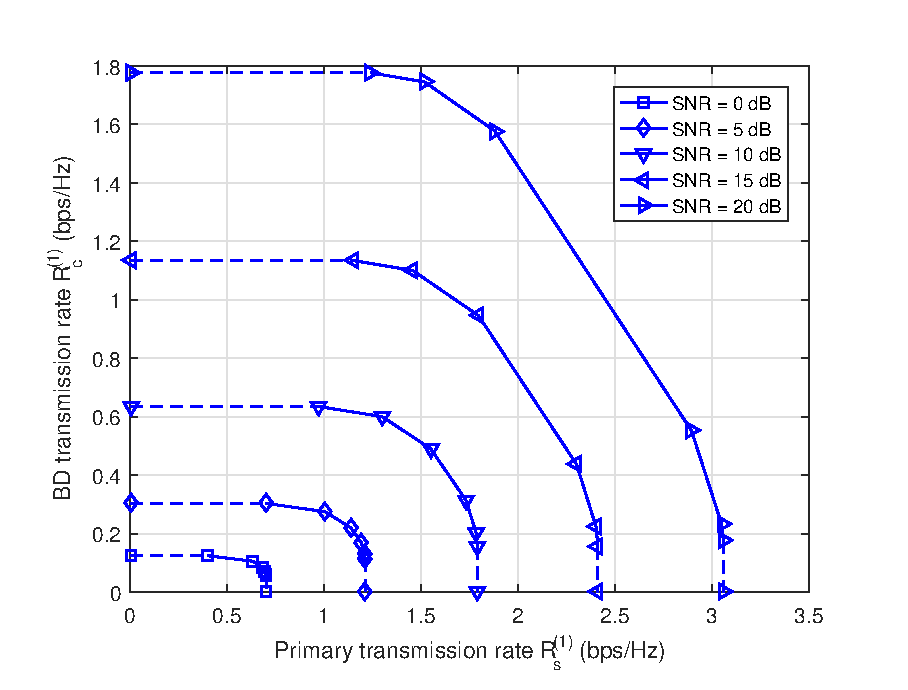
\includegraphics[width=0.7\textwidth]{assets/psr_region.eps}
					\caption{Rate region of PSR \cite{Long2019a}}
					\label{fi:psr_region}
				\end{figure}
			\end{frame}

			\begin{frame}{TPM: Transmit Power}
				\begin{figure}
					\centering
					\begin{subfigure}{.45\textwidth}
						\centering
						\includegraphics[width=\linewidth]{assets/psr_power_rc.eps}
						\caption{PSR ($N=1$)}
					\end{subfigure}
					\begin{subfigure}{.45\textwidth}
						\centering
						\includegraphics[width=\linewidth]{assets/csr_power_rc.eps}
						\caption{CSR ($N=128$)}
					\end{subfigure}
					\caption{Minimum transmit power $P$ vs backscatter rate constraint $\epsilon_c$}
				\end{figure}
			\end{frame}

			\begin{frame}{TPM: Rate Tradeoff}
				\begin{figure}
					\centering
					\begin{subfigure}{.48\textwidth}
						\centering
						\includegraphics[width=0.8\linewidth]{assets/psr_rs_rc.eps}
						\caption{PSR: primary rate $R_{s}^{\text{PSR}}$ vs backscatter rate constraint $\epsilon_c$}
					\end{subfigure}
					\begin{subfigure}{.48\textwidth}
						\centering
						\includegraphics[width=0.8\linewidth]{assets/psr_rc_rs.eps}
						\caption{PSR: secondary rate $R_{c}^{\text{PSR}}$ vs primary rate constraint $\epsilon_s$}
					\end{subfigure}
					\begin{subfigure}{.48\textwidth}
						\centering
						\includegraphics[width=0.8\linewidth]{assets/csr_rs_rc.eps}
						\caption{CSR: primary rate $R_{s}^{\text{CSR}}$ vs backscatter rate constraint $\epsilon_c$}
					\end{subfigure}
					\begin{subfigure}{.48\textwidth}
						\centering
						\includegraphics[width=0.8\linewidth]{assets/csr_rc_rs.eps}
						\caption{CSR: secondary rate $R_{c}^{\text{CSR}}$ vs primary rate constraint $\epsilon_s$}
					\end{subfigure}
				\end{figure}
			\end{frame}
		\end{subsection}

		\begin{subsection}{Limitations and Opportunities}
			\begin{frame}{Limitations and Opportunities}
				Limitations:
				\begin{itemize}
					\item \textbf{Channel model:} double fading may not cover backscatter channel properties as rank deficiency and channel correlation.
					\item \textbf{Channel estimation:} need carefully designed pilots and low complexity algorithms.
					\item \textbf{Synchronization:} traditional solution requires power-consuming oscillators at the backscatter device.
					\item \textbf{Security:} the secondary transmission relies heavily on the primary transmission.
				\end{itemize}

				\vspace{1em}

				Opportunities:
				\begin{itemize}
					\item Integrate the IRS reflection coefficient $\boldsymbol{\phi}$ and the backscatter message $c$ for multi-antenna backscatter?
					\item Design SR in broadcasting and multiple access systems?
					\item Suppress the backscatter signal at other frequencies?
				\end{itemize}
			\end{frame}
		\end{subsection}
	\end{section}

	\bibliographystyle{IEEEtran}
	\bibliography{IEEEabrv,library.bib}
\end{document}
